\chapter{Implementation}

Implementations in the C programming language for the presented strategies can
be found in Appendix \ref{app:cimpl}. Although directly writing Assembler code
could result in a small performance benefit, this generally increases the work
necessary by an order of magnitude for only limited results. Instruction-level
optimization and in particular register allocation is left to the compiler.
Relying on the compiler mandates a closer study of the generated, optimized
assembler. All source files were compiled using clang version 15.0.7 and
optimization level O3.

\section{Pipelining}

Understanding certain choices requires an understanding of the Cortex-A73
instruction pipeline \cite{a72opt:2015}. Being a superscalar processor, it is
able to execute more than one instruction per clock cycle by dispatching
instructions to different execution units working in parallel.

\begin{figure}{h!}
    \centering
    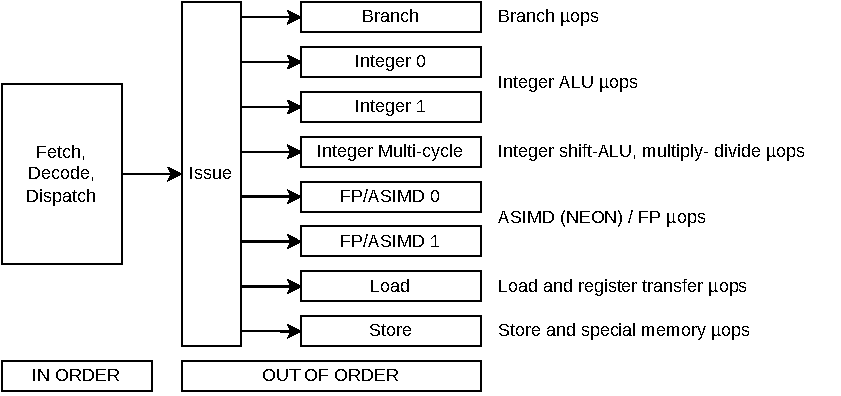
\includegraphics[width=0.7\textwidth]{Figures/a72pipeline.pdf}
    \caption{High-level overview of the Cortex-A72 instruction pipeline}
\end{figure}

The processor might for example store a calculation result, load a necessary
value from memory and execute two SIMD operations at once, all in the same
clock cycle. Modern compilers take advantage of this fact by reordering
instructions such that all pipeline execution units stay as busy as possible
and do not stall while having to wait for new instructions to be dispatched. A
more thorough analysis will be presented for the bitsliced strategy of
\texttt{GIFT}, but all implementations are heavily reliant on function
inlining, instruction reordering and loop unrolling.

\section{GIFT}
\subsection{Table-based}

This is the simplest strategy to implement. Indeed, its biggest advantage lies
in its portability to other platforms without relying on specific features or
extensions. The cipher state is stored as a 64-bit word and one round consists
in extracting the 4-bit S-boxes, looking up table values, collecting these in
an accumulator and finally adding the round key.

\lstinputlisting[language=c, caption={GIFT-64 table subperm}, firstline=77, lastline=87]{../impl/gift/table.c}
\lstinputlisting[language=c, caption={GIFT-64 table encrypt}, firstline=89, lastline=101]{../impl/gift/table.c}

Lots of operations require extraction of a certain number of consecutive bits,
usually referred to as a bitfield. Indices for table lookups are generally
attained by right-shifting a larger value stored in a register, then applying
an AND operation to get the lowest $n$ bits and finally writing the result into
the beginning of another register. Due to its usefulness, this operation is
implemented as \texttt{UBFX} for an unsigned bitfield extract and can be used
to implement S-box extraction for subperm lookups which would otherwise take
two or three instructions. Interestingly, the AArch64 instruction set makes
heavy use of instruction aliasing. The logical shift left instruction
\texttt{lsl} for example is an alias of \texttt{UBFX} which itself is an alias
for \texttt{UBFM}.

Another keyword aiding in optimization is \texttt{restrict} which can be used
for pointer and array function parameters; the programmer can add this keyword
to parameters to tell the compiler they are never aliased by any other pointers
which allows the compiler to rearrange instructions and eliminate loads.

\subsection{Using \texttt{vperm}}

Implementation of the substitution layer requires the use of a single vector
intrinsic. This mandates the packing of data into a vector register which in
turn is disadvantageous to the permutation layer as we need to extract single
bits. Packing and unpacking is nothing more than filling 8-bit vector lanes
with 4-bit S-boxes and vice versa.

\lstinputlisting[language=c, caption={\texttt{vperm} S-box}, firstline=95, lastline=98]{../impl/gift/vec_sbox.c}
\lstinputlisting[language=c, caption={\texttt{vperm} permutation}, firstline=105, lastline=120]{../impl/gift/vec_sbox.c}
\lstinputlisting[language=c, caption={\texttt{vperm} encrypt function}, firstline=200, lastline=215]{../impl/gift/vec_sbox.c}

\subsection{Bitslicing}

\subsubsection{A note on data storage}

NEON only provides 32 vector registers. While this is more than the 16 YMM
registers offered by Intel's AVX-256 vector extension, it is not enough to
accompany all 28 round keys for GIFT-64 plus the 16 registers representing
cipher state at once. Because loading and storing single registers is
inefficient, data is represented using the vector array type
\texttt{uint8x16x4\_t}. Loads and stores are then assembled such that the whole
array is loaded or stored in a single instruction. Loading a single vector from
memory for example has a latency of 5 cycles while loading four vectors into a
vector array can be done in 8 cycles which results in an amortized cost of 2
cycles per vector. Vectors are grouped into vector arrays as often as possible
to reduce the number of necessary loads and stores.

\subsubsection{Shifts for swapmove}

Implementing shift functions for 128-bit NEON registers by extracting the
overflow and adding it back in later can be realized using 5 instructions. It
would be most useful for the function to take a shift amount parameter, but
most NEON intrinsics encode their parameters into the final machine code such
that parameters need to be compile-time constants. We will therefore implement
\texttt{shl}, \texttt{shr} and \texttt{swapmove} as C macros utilizing the
\texttt{vextq\_u64} intrinsic to swap the two 64-bit vector elements:

\lstinputlisting[language=c, caption={Bitsliced GIFT swapmove and shift macros}, firstline=50, lastline=79]{../impl/gift/vec_sliced.c}

\subsubsection{Round function}
We will examine the round function in closer detail and compare the source code
with the generated assembly.

\lstinputlisting[language=c, caption={Bitsliced GIFT S-box}, firstline=157, lastline=180]{../impl/gift/vec_sliced.c}
\lstinputlisting[language=c, caption={Bitsliced GIFT permutation}, firstline=205, lastline=216]{../impl/gift/vec_sliced.c}

\begin{lstlisting}[language=c, caption={Round function}]
for (int round = 0; round < ROUNDS_GIFT_64; round++) {
    gift_64_vec_sliced_subcells(s);
    gift_64_vec_sliced_permute(s);

    // round key addition
    s[0].val[0] = veorq_u8(s[0].val[0], rks[round][0].val[0]);
    s[0].val[1] = veorq_u8(s[0].val[1], rks[round][0].val[1]);
    s[0].val[2] = veorq_u8(s[0].val[2], rks[round][0].val[2]);
    s[0].val[3] = veorq_u8(s[0].val[3], rks[round][0].val[3]);
    s[1].val[0] = veorq_u8(s[1].val[0], rks[round][1].val[0]);
    s[1].val[1] = veorq_u8(s[1].val[1], rks[round][1].val[1]);
    s[1].val[2] = veorq_u8(s[1].val[2], rks[round][1].val[2]);
    s[1].val[3] = veorq_u8(s[1].val[3], rks[round][1].val[3]);
}
\end{lstlisting}

\begin{minipage}{.45\textwidth}
    \begin{lstlisting}[language={[ARM]Assembler}, caption={Round function asm}, escapechar=|]
and     v20.16b, v17.16b, v6.16b
add     x9, x20, x8
eor     v20.16b, v20.16b, v16.16b
add     x8, x8, #0x80|\label{lst:cntrincr}|
and     v21.16b, v20.16b, v19.16b
cmp     x8, #0xe70|\label{lst:cntrchk}|
eor     v21.16b, v21.16b, v6.16b
orr     v6.16b, v6.16b, v16.16b
eor     v6.16b, v6.16b, v17.16b
eor     v16.16b, v19.16b, v6.16b
eor     v17.16b, v16.16b, v20.16b
and     v19.16b, v21.16b, v17.16b
eor     v6.16b, v19.16b, v6.16b
and     v19.16b, v7.16b, v4.16b
eor     v19.16b, v19.16b, v5.16b
and     v20.16b, v19.16b, v18.16b
eor     v20.16b, v20.16b, v4.16b
orr     v4.16b, v4.16b, v5.16b
eor     v4.16b, v4.16b, v7.16b
eor     v5.16b, v18.16b, v4.16b
eor     v7.16b, v5.16b, v19.16b
and     v18.16b, v20.16b, v7.16b
eor     v4.16b, v18.16b, v4.16b
    \end{lstlisting}
\end{minipage}\hfill
\begin{minipage}{.45\textwidth}
    \vspace*{7mm}
    \begin{lstlisting}[language={[ARM]Assembler}, firstnumber=24, escapechar=|]
tbl     v18.16b, {v6.16b}, v2.16b
tbl     v19.16b, {v21.16b}, v3.16b
tbl     v21.16b, {v4.16b}, v2.16b
ldp     q6, q4, [x9, #-112]|\label{lst:floatload}|
mvn     v16.16b, v16.16b
tbl     v16.16b, {v16.16b}, v0.16b
tbl     v17.16b, {v17.16b}, v1.16b
mvn     v5.16b, v5.16b
tbl     v5.16b, {v5.16b}, v0.16b
ldp     q22, q23, [x9, #-80]
eor     v6.16b, v6.16b, v16.16b
eor     v16.16b, v4.16b, v17.16b
tbl     v7.16b, {v7.16b}, v1.16b
eor     v17.16b, v22.16b, v18.16b
tbl     v20.16b, {v20.16b}, v3.16b
ldp     q4, q18, [x9, #-48]
eor     v19.16b, v23.16b, v19.16b
eor     v4.16b, v4.16b, v5.16b
ldp     q22, q23, [x9, #-16]
eor     v5.16b, v18.16b, v7.16b
eor     v7.16b, v22.16b, v21.16b
eor     v18.16b, v23.16b, v20.16b
b.ne    197e0
    \end{lstlisting}
\end{minipage}

It is obvious to see the compiler has inlined the two function calls to
\texttt{subcells} and \texttt{permute} with lines 1 to 23 originating from the
\texttt{subcells} and lines 24-46 from the \texttt{permute} and round key
addition functions. It has chosen not to unroll the loop, but has moved the
loop counter increment as well as the condition check in between the
\texttt{subcells} instructions to line \ref{lst:cntrincr} and
\ref{lst:cntrchk}. In addition, the loop counter serves a second purpose as an
offset register and is therefore incremented by 0x80=128 instead of just 1.

Permutation (\texttt{tbl}) and round key addition (\texttt{eor}) instructions
are interleaved. The compiler recognizes data dependencies and can therefore
proceed with round key addition immediately after a slice has been permuted
without needing to wait for all permutations to finish. This is only logical
considering the inner workings of the instruction pipeline: by interleaving
NEON with regular logic and load instructions, the execution units are filled
more evenly and pipeline stalls are prevented which speeds up computation.

Round keys are loaded from memory a few instructions before they are needed;
assuming all round keys are stored in the L1 cache, loading a
floating-point/vector register takes 5 cycles. After the load has been
dispatched to the load execution unit in line \ref{lst:floatload}, the
processor continues processing the instruction stream by issuing \texttt{tbl}
and \texttt{mvn} $\mu$ops to other execution units.

These kinds of optimizations are pervasive when programming using higher level
languages like C and modern-day compilers more often than not outperform
handcrafted assembly.

\section{Camellia}
\subsection{Optimized non-SIMD implementation}

An optimized non-SIMD implementation based on the platform-independent
techniques presented in the original paper is relatively easy to achieve since
all functional components are already well defined. One thing to take note of
however is the fact that the specification is based on a big endian
representation while ARMv8 is a little endian machine. The problem of
endianness manifests itself whenever a memory-register interaction takes place,
i.e. for loads and stores. Arithmetic on a register is unaffected since a
register is always treated as one large number with no conception of addresses.

We will store input data and arrays in Camellia byte-order such that a lower
array element actually represents a higher numerical value, i.e. the numerical
value of

\begin{center}
    \texttt{\{ 0x0123456789abcdefUL, 0xfedcba9876543210UL \}}
\end{center}

is equal to

\begin{center}
    \texttt{0x0123456789abcdeffedcba9876543210}
\end{center}

which is equal to the byte string

\begin{center}
    \texttt{01 23 45 67 89 ab cd ef fe dc ba 98 76 54 32 10}
\end{center}

This allows us to change the endianness of the implementation while keeping
input in the original Camellia byte order. A change in implementation
endianness manifest itself for example in table lookups where, according to
Camellia specification, the first byte is expected to be the most significant
byte:

\lstinputlisting[language=c, caption={Camellia optimized SP function with reverse byte order}, firstline=29, lastline=45]{../impl/camellia/spec_opt.c}

\subsection{Bytesliced implementation}

\subsubsection{Key generation}

A possible approach to storing keys is storing them in bytesliced format so
they can later be loaded from memory and used directly since we only have 32
vector registers in total and half of them are already occupied by the current
cipher state. This can be implemented by first generating 64 bit round keys and
then filling register $V_i$ with the $i$-th byte by means of
\texttt{vdupq\_n\_u8} for each key.

\lstinputlisting[language=c, caption={Bytesliced Camellia round key generation}, firstline=237, lastline=266]{../impl/camellia/bytesliced.c}

Another way to implement key generation is not to store the keys bytesliced,
but rather to store the 64 bit values and create necessary vector registers on
the fly. This saves 3120 bytes of memory and could show some usefulness for
memory-constrained environments, but benchmarking shows a performance drop of
about $3.6\%$. This is due to the fact that \texttt{vdupq\_n\_u8} has a latency
of 8 cycles and a throughput of only 1, making it a great deal slower than
simple vector array loads.

\subsubsection{F-function}

The s-function implements matrix multiplication with a given pre- and
postfilter using the aforementioned strategy.

\lstinputlisting[language=c, caption={Bytesliced Camellia S-box}, firstline=40, lastline=65]{../impl/camellia/bytesliced.c}

Just as before we need to invert the byte order since the first vector
\texttt{X[0].val[0]} contains all least significant bytes, but the Camellia
specification places the most significant bytes at the beginning.

\lstinputlisting[language=c, caption={Bytesliced Camellia F-function}, firstline=67, lastline=109]{../impl/camellia/bytesliced.c}
